\subsection{Working with 2D List}
\subsubsection{2D List indexes}
When working with 2D List, its indexes are commonly divided into 2 categories:
\begin{itemize}
	\item Row Index.
	\item Column Index.
\end{itemize}
\newpage

\begin{figure}[h]
	\centering
	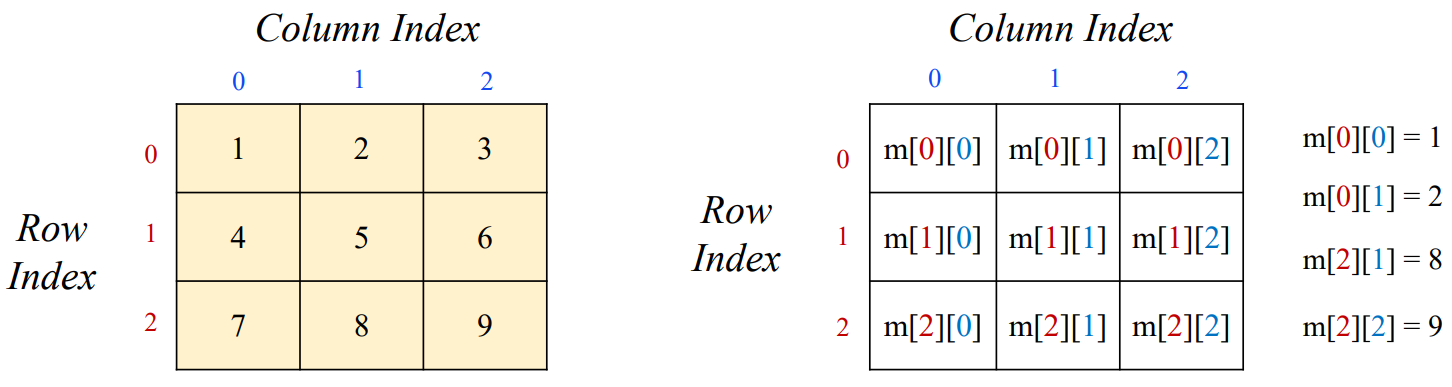
\includegraphics[width=1.0\textwidth]{2dlist-index}
	\caption{Row indexes and Column indexes}
	\label{fig:2dindex}
\end{figure}

\subsubsection{Create 2D List}
	\begin{center}
		m = [[1, 2, 3], [4, 5, 6], [7, 8, 9]]
	\end{center}

\subsubsection{Accessing Elements}
	\begin{center}
		m[r][c]: the value at row r and column c.
	\end{center}
	
\subsubsection{Iterating over a 2D Matrix}
\noindent
\begin{minipage}[c]{0.55\textwidth}
	\begin{itemize}
		\item Sol 1:
			\begin{verbatim}
				for row in m:
					for element in row:
						print(element, end=' ')
					print()
			\end{verbatim}
		\item Sol 2:
			\begin{verbatim}
				for r in range(num_rows):
					for c in range(num_cols):
						print(m[r][c], end=' ')
					print()
			\end{verbatim}
	\end{itemize}
\end{minipage}%
\hfill
\begin{minipage}[t]{0.4\textwidth}
	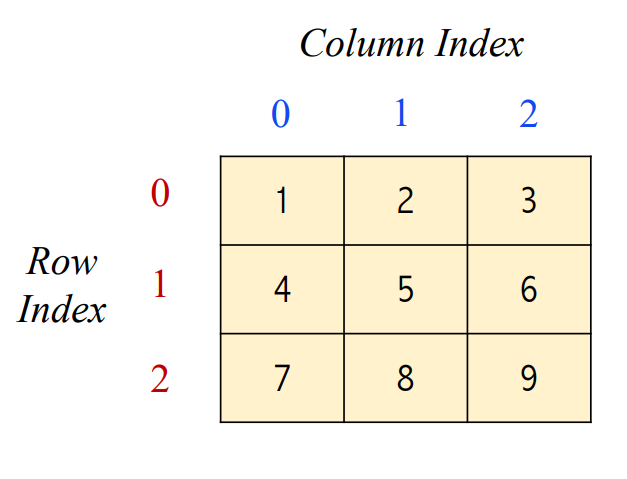
\includegraphics[width=\linewidth]{matrix-index}
\end{minipage}


\subsubsection{Update elements in 2D matrix}
\begin{center}
	\begin{verbatim}
		matrix[r][c] = new_value
	\end{verbatim}
\end{center}